\section{How do the different layers of a CNN train over time? How much pretraining is sufficient?}
\label{sec:speed}
Training CNNs is very time consuming. \cite{Kriz} trained for around 7 days for achieving state of art results on Imagenet. Even finetuning for PASCAL object detection \cite{Rcnn} takes over 12 hours on the advanced GPUs such as the Nvidia Tesla-K40. This is a big barrier towards exploring different network architectures. Layerwise training has been previously used for learning parameters of multilayer networks(REF). We hypothesized, that maybe such methods which train one layer at a time can be used to speed-up CNN training. Before, testing this we sought to determine if simultaneous learning of parameters in all layers of CNNs by itself proceeds in a layerwise manner. 


\setlength{\tabcolsep}{4pt}
\begin{table}[t!]
\begin{center}
\caption{Variation in classification accuracy (mean-AP) on PASCAL VOC 2007 challenge using features extracted from different layers of Alex-Net as a function of number of iterations.}
\label{table:det-traj-classify}
\begin{tabular}{lcccccccc}
\hline\noalign{\smallskip}
Layer  & 5K & 15K & 25K & 35K & 45K & 95K & 105K & 310K \\
\noalign{\smallskip}
\hline
\noalign{\smallskip}
conv-1 & 23.0 & 24.3 & 24.4 & 24.5 & 24.6 & 24.8 & 24.7 & 25.1\\
conv-2 & 33.7 & 40.4 & 40.9 & 41.8 & 42.0 & 43.2 & 44.0 & 45.0\\
conv-3 & 34.2 & 46.8 & 47.0 & 48.2 & 48.5 & 49.4 & 51.6 & 50.1\\
conv-4 & 33.5 & 49.0 & 48.7 & 50.2 & 50.6 & 51.6 & 54.1 & 54.2\\
conv-5 & 33.0 & 53.4 & 55.0 & 56.8 & 57.4 & 59.2 & 63.5 & 65.6\\
fc-6 & 34.2 & 59.7 & 62.6 & 62.7 & 64.1 & 65.6 & 69.3 & 70.6\\
fc-7 & 30.9 & 61.3 & 64.1 & 65.1 & 65.8 & 67.8 & 71.8 & 73.2\\
\hline
\end{tabular}
\end{center}
\end{table}
\setlength{\tabcolsep}{1.4pt}

\begin{figure}[t!]
\centering
\subfloat[5K Iterations]{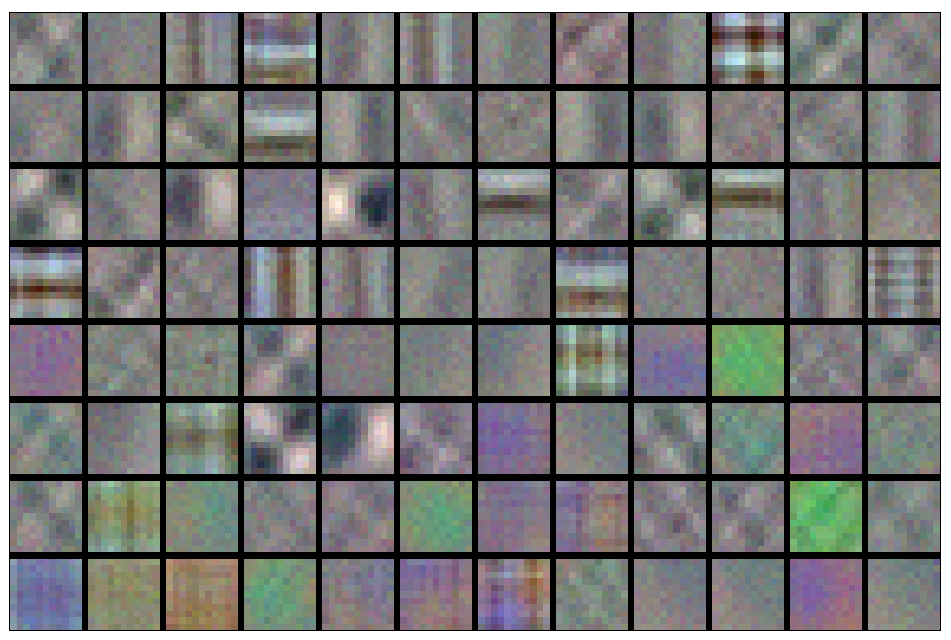
\includegraphics[scale=0.10]{images/l1_filters_iter5000.png}} \hspace{2mm}
\subfloat[15K Iterations]{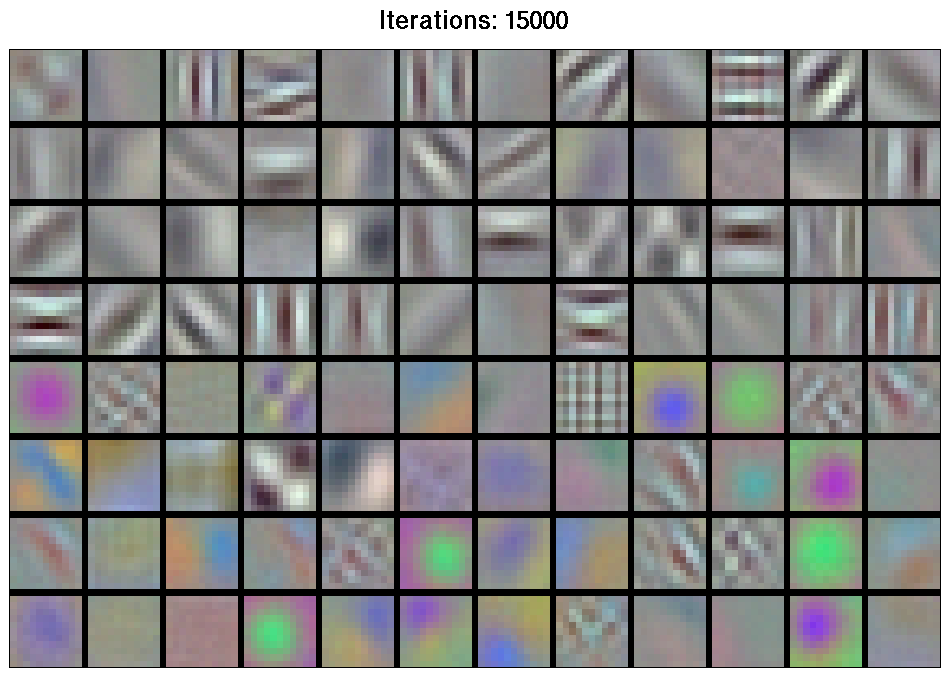
\includegraphics[scale=0.10]{images/l1_filters_iter15000.png}} \hspace{2mm}
\subfloat[225K Iterations]{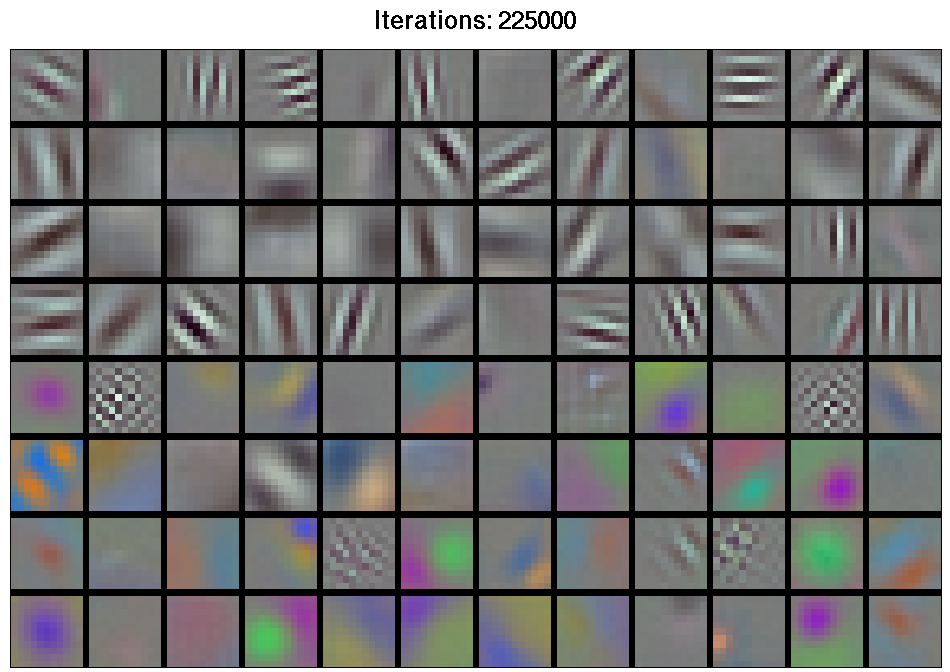
\includegraphics[scale=0.10]{images/l1_filters_iter225000.png}}
\caption{(a),(b),(c) show conv-1 filters after 5K, 15K and 225K iterations of training respectively. One pass (epoch) over the entire Imagenet-ILSVRC12 dataset takes approximately 5K iterations. Notice, that just after 15K iterations these filters closely resemble their final state.}
\label{fig:conv1}
\end{figure}

For probing this, linear SVM was trained for PASCAL 2007 image classification using features extracted from individual layers. The results are summarized in table \ref{table:det-traj-classify}.It is quite surprising to note that by 15K iterations all layers are within 80\% and at 50K iterations within 90\% of there final performance. This strongly indicates that a great portion of training required for generalization happens quite quickly. 

Motivated by these observations we trained a 50-50 network (50K iterations on imagenet and finetuned for 50K iterations using the procedure described in sec. \ref{sub:fine-train}) and evaluated its performance on the  Pascal 2007 detection challenge (see table \ref{table:det-trajectory} for results). Consistent with our earlier results we find that this network achieves a surprising performance of 48.6 mean AP points compared to 54.1 achieved by pre-training for 310K iterations. 

\setlength{\tabcolsep}{1pt}
\begin{table}[t!]
\begin{center}
\caption{Performance of 50-50 network for detection on pascal-voc-2007 challenge. (l5 is conv-5 and l7 is fc-7)}
\label{table:det-trajectory}
\scalebox{1.00}{
\begin{tabular}{|l|cccc|}
\hline
 & 50K & 105K & 205K & 305K \\
\hline
det & - & - & - & - \\
sun-397 & - & - & - & - \\
\hline
\end{tabular}}
\end{center}
\end{table}
\setlength{\tabcolsep}{1.4pt}
The above analysis reinforces our belief that indeed majority of training required for generalization happens quite quickly as compared to the full training time of the network. This observation suggest that there may exist clever ways which can help us speed up the training.

